\documentclass{article}
\usepackage[utf8]{inputenc}
\usepackage{enumitem}
\usepackage{graphicx}

\title{Reeksamen 2015}
\author{kiettn12}
\date{November 2020}

\begin{document}

\maketitle
\title{
\normalsize \normalfont
\textbf{Opgave 1}}
\\
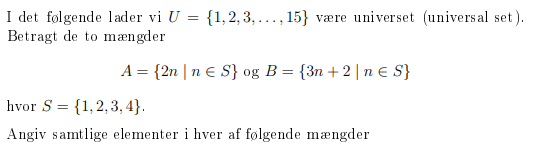
\includegraphics[width=1.0 \textwidth]{Reeksamen.PNG}
\begin{enumerate}[label=(\Alph*)]
\item $A
\\
$A = \big\{2,4,6,8\big\}
\\

\item $B 
\\
$B = \big\{5,8,11,14\big\}
\\

\item $A \cap $B 
\\
$A \cap $B = \big\{8\big\}
\\

\item $A\cup$B 
\\
$A\cup$B = \big\{2,4,5,6,8,11,13\big\}
\\

\item $A-B$
\\
A-B= \big\{2,4,6\big\}
\\

\item \overline{A}
\\ 
\overline{A} = \big\{1,3,5,7,9,10,11,12,13,14,15\big\}
\\

\end{enumerate}
\\

\end{document}
